\documentclass{../../text-style}

\texttitle{Лекция 2: О жизненном цикле и методологиях}

\begin{document}

\maketitle
\thispagestyle{empty}

\attribution{Тимофей Александрович Брыксин, бывш. доцент кафедры системного программирования СПбГУ}

\section{Жизненный цикл программного обеспечения}

В первой лекции говорилось о том, что сложную программную систему построить <<простыми>> методами невозможно. Ее разработка с неизбежностью будет тоже сложной деятельностью. Привести такое дело к успеху возможно на основе общих принципов работы со сложными системами: организовав его в виде набора компонент, используя разные уровни абстракции. Выделить компоненты можно, определив набор задач, которые нужно решить для достижения конечной цели. Для решения каждой такой задачи организуется вспомогательная деятельность, к которой можно также применить декомпозицию на отдельные, более мелкие деятельности, и т.д.

В качестве примеров деятельностей, которые нужно проводить для построения программной системы, можно привести проектирование~--- выделение отдельных модулей и определение связей между ними с целью минимизации зависимостей между частями проекта и достижения лучшей его обозримости в целом; кодирование~--- разработку кода отдельных модулей; разработку пользовательской документации, которая необходима для достаточно сложной системы. Однако для корректного с точки зрения инженерии и экономики рассмотрения вопросов создания сложных систем необходимо, чтобы были затронуты и вопросы эксплуатации системы, внесения в нее изменений, а также самые первые действия в ходе ее создания~--- анализ потребностей пользователей и выработка решений, <<изобретение>> функций, удовлетворяющих эти потребности. Без этого невозможно, с одной стороны, учесть реальную эффективность системы в виде отношения полученных результатов ко всем сделанным затратам и, с другой стороны, правильно оценивать в ходе разработки степень соответствия системы реальным нуждам пользователей и заказчиков.

Весь период существования ПО, связанный с подготовкой к его разработке, разработкой, использованием и модификациями, начиная с того момента, когда принимается решение разработать/приобрести/собрать из имеющихся компонентов новую систему, или приходит сама идея о необходимости программы определенного рода, до того момента, когда полностью прекращается всякое ее использование, называют \emph{жизненным циклом ПО}.

В ходе жизненного цикла создаются и перерабатываются различного рода артефакты~--- создаваемые человеком информационные сущности, документы в достаточно общем смысле, участвующие в качестве входных данных и получающиеся в качестве результатов различных деятельностей. Примерами артефактов являются: модель предметной области, описание требований, техническое задание, архитектура системы, проектная документация на систему в целом и на ее компоненты, прототипы системы и компонентов, собственно, исходный код, пользовательская документация, документация администратора системы, руководство по развертыванию, база пользовательских запросов, план проекта, и пр.

На различных этапах в создание и эксплуатацию ПО вовлекаются люди, выполняющие различные роли. Каждая роль может быть охарактеризована как абстрактная группа заинтересованных лиц, участвующих в деятельности по созданию и эксплуатации системы и решающих одни и те же задачи или имеющих одни и те же интересы по отношению к ней. Примерами ролей являются: бизнес-аналитик, инженер по требованиям, архитектор, проектировщик пользовательского интерфейса, программист-кодировщик, технический писатель, тестировщик, руководитель проекта по разработке, работник отдела продаж, конечный пользователь, администратор системы, инженер по поддержке и т.п.

Похоже, что общую структуру жизненного цикла любого ПО задать невозможно, поскольку она существенно зависит от целей, для которых это ПО разрабатывается или приобретается, и от решаемых им задач. Тем не менее, часто определяют основные элементы структуры жизненного цикла в виде \emph{модели жизненного цикла ПО}. Модель жизненного цикла ПО выделяет конкретные наборы видов деятельности (обычно разбиваемых на еще более мелкие активности), артефактов, ролей и их взаимосвязи, а также дает рекомендации по организации процесса в целом. Эти рекомендации включают ответы на вопросы о том, какие артефакты являются входными данными у каких видов деятельности, а какие появляются в качестве результатов, какие роли вовлечены в различные деятельности, как различные деятельности связаны друг с другом, каковы критерии качества полученных результатов, как оценить степень соответствия различных артефактов общим задачам проекта и когда можно переходить от одной деятельности к другой и т.д.

Стоит отметить, что идея модели процесса появилась в программной инженерии очень давно, в те времена, когда считалось, что удачная модель~--- самое главное, что способствует успеху разработки. Позднее пришло осознание, что существует множество других аспектов (принципы управления и разработки, структура команды и т.д.), которые должны быть определены согласованно друг с другом.

\section{Модели жизненного цикла}

\subsection{Водопадная модель}
 
Наиболее широко известной и применяемой долгое время оставалась так называемая каскадная или водопадная (waterfall) модель жизненного цикла, которая, как считается, впервые четко сформулирована в 1970 году Винстоном Ройсом в работе <<Managing the Development of Large Software Systems>>\footnote{\url{http://www-scf.usc.edu/~csci201/lectures/Lecture11/royce1970.pdf} (дата обращения: 25.02.2022).} и впоследствии запечатлена в стандартах министерства обороны США в семидесятых-восьмидесятых годах XX века. Эта модель предполагает последовательное выполнение различных видов деятельности, начиная с выработки требований и заканчивая сопровождением, с четким определением границ между этапами, на которых набор документов, созданный на предыдущей стадии, передается в качестве входных данных для следующей. Таким образом, каждый вид деятельности выполняется на какой-то одной фазе жизненного цикла. <<Классическая>> каскадная модель предполагает только движение вперед по этой схеме: все необходимое для проведения очередной деятельности должно быть подготовлено в ходе предшествующих работ. Отмечалось, что возвраты могут катастрофически увеличить стоимость проекта и сроки его выполнения. Например, если при тестировании обнаруживаются ошибки проектирования или анализа, то их исправление часто приводит к полной переделке системы. Этой моделью допускались возвраты только на предыдущий шаг: например, от тестирования к кодированию, от кодирования к проектированию и т.д.

\begin{center}
    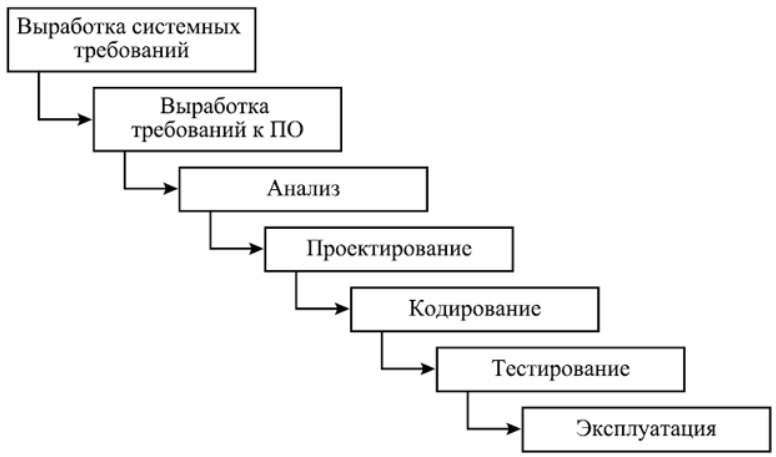
\includegraphics[width=0.7\textwidth]{waterfall.png}
\end{center}

Ещё в рамках этой модели (и об этом редко говорят) было введено прототипирование, то есть предлагалось разрабатывать систему дважды, чтобы уменьшить риски разработки. Первая версия~--- прототип~--- позволяет увидеть основные риски и обоснованно принять главные архитектурные решения, оценить технические ограничения. На создание прототипа отводилось до одной трети времени всей разработки. Также Ройс настаивает на непосредственном вовлечении заказчика в процесс разработки. Это требование мы будем встречать и в последующих моделях жизненного цикла.

\begin{center}
    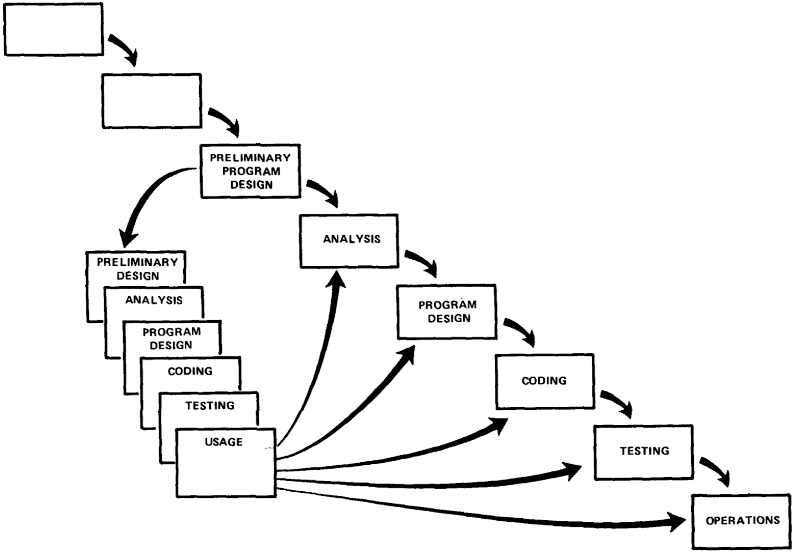
\includegraphics[width=0.7\textwidth]{waterfallPrototyping.png}
\end{center}

В качестве плюсов данной модели можно отметить относительную простоту планирования проекта (чёткие этапы с чёткими границами). Также на разных этапах нужны разные специалисты, а значит, их можно привлекать лишь на определённое время.

Работать в соответствии с этой моделью можно, только если удается предвидеть заранее возможные особенности хода проекта и тщательно собирать и анализировать информацию на первых этапах, с тем, чтобы впоследствии можно было пользоваться их результатами без оглядки на возможные изменения.

Сейчас данная модель продолжает использоваться на практике~--- для небольших, простых проектов, в хорошо формализованных проектах (и в тех, и в других есть чётко определённое ТЗ, которое вряд ли будет меняться) или при разработке типовых систем, где итеративность не так востребована. С ее помощью удобно отслеживать разработку и осуществлять поэтапный контроль за проектом.

\subsection{Инкрементально-итеративные модели}

Среди разработчиков и исследователей, имевших дело с разработкой сложного ПО, практически с самого зарождения индустрии производства программ (см., например, статью 1968 года \url{https://www.researchgate.net/publication/221329933_Iterative_Multi-Level_Modeling_-_A_Methodology_for_Computer_System_Design} (дата обращения: 25.02.2023)) большую популярность имели модели эволюционных или итеративных процессов, поскольку они обладают большей гибкостью и способностью работать в меняющемся окружении. Итеративные или инкрементальные модели (известно несколько таких моделей) предполагают разбиение создаваемой системы на набор кусков, которые разрабатываются с помощью нескольких последовательных проходов всех работ или их части. На первой итерации разрабатывается кусок системы, не зависящий от других. При этом большая часть или даже полный цикл работ проходится на нем, затем оцениваются результаты и на следующей итерации либо первый кусок переделывается, либо разрабатывается следующий, который может зависеть от первого, либо как-то совмещается доработка первого куска с добавлением новых функций. В результате на каждой итерации можно анализировать промежуточные результаты работ и реакцию на них всех заинтересованных лиц, включая пользователей, и вносить корректирующие изменения на следующих итерациях. Каждая итерация может содержать полный набор видов деятельности от анализа требований, до ввода в эксплуатацию очередной части ПО. 

\begin{center}
    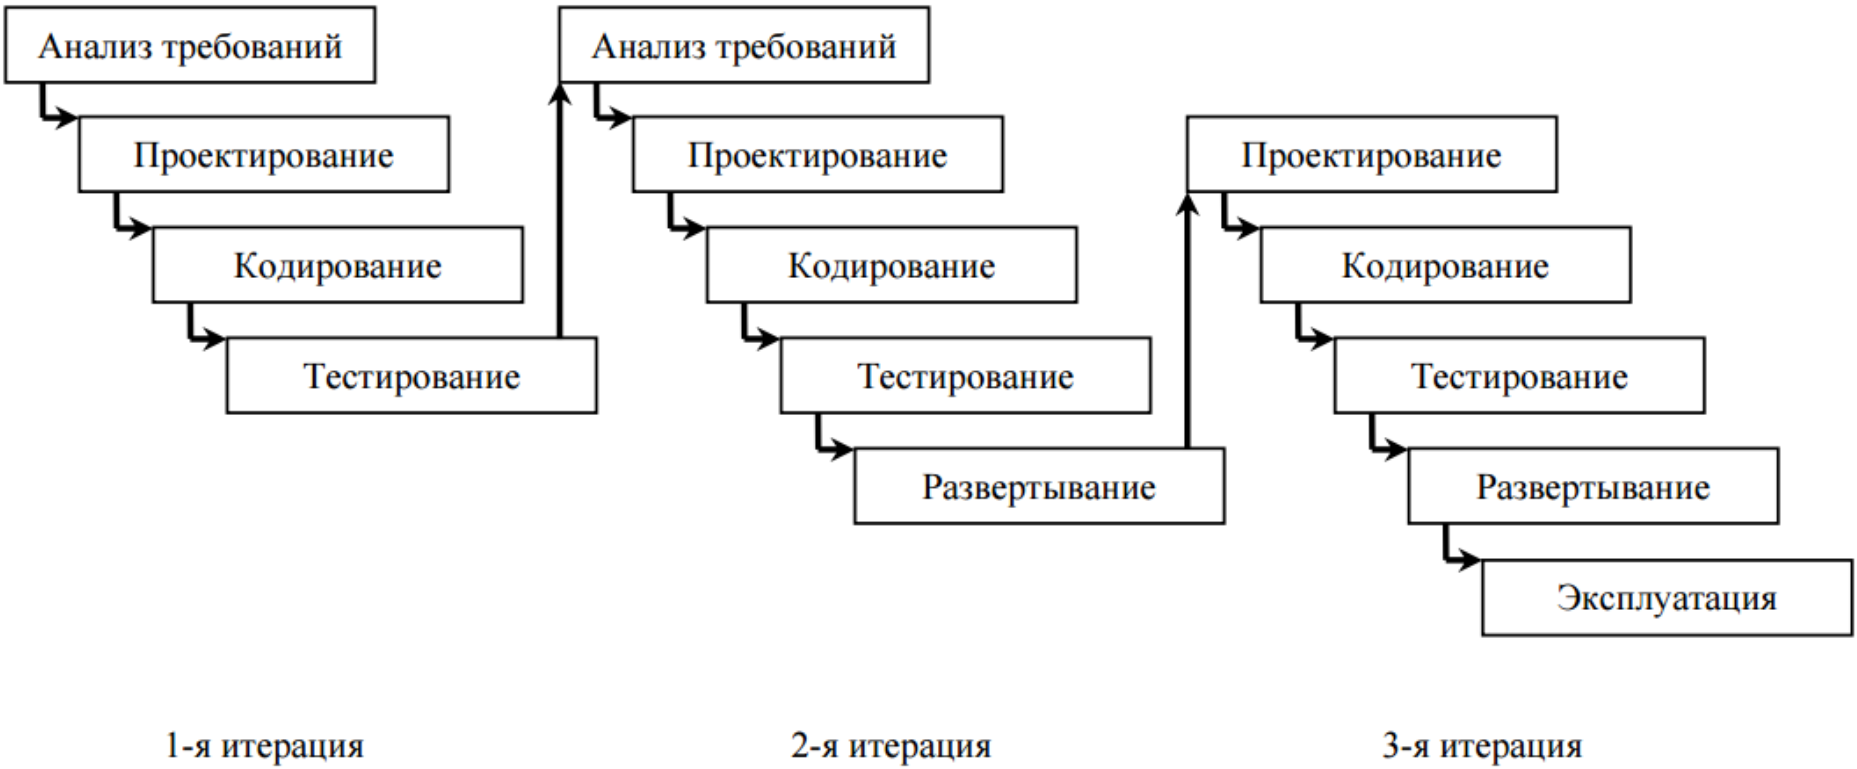
\includegraphics[width=0.8\textwidth]{iterativeModel.png}
\end{center}

Итеративный процесс предполагает, что разные виды деятельности не привязаны намертво к определенным этапам разработки, а выполняются по мере необходимости, иногда повторяются, до тех пор, пока не будет получен нужный результат. Вместе с гибкостью и возможностью быстро реагировать на изменения, итеративные модели привносят дополнительные сложности в управление проектом и отслеживание его хода. При использовании итеративного подхода значительно сложнее становится адекватно оценить текущее состояние проекта и спланировать долгосрочное развитие событий, а также предсказать сроки и ресурсы, необходимые для обеспечения определенного качества результата.

Развитием идеи итераций является спиральная модель жизненного цикла ПО, предложенная Боэмом в 1988 году\footnote{\url{http://csse.usc.edu/TECHRPTS/1988/usccse88-500/usccse88-500.pdf} (дата обращения: 25.02.2023).}. Она предлагает каждую итерацию начинать с выделения целей и планирования очередной итерации, определения основных альтернатив и ограничений при ее выполнении, их оценки, а также оценки возникающих рисков и определения способов избавления от них, а заканчивать итерацию оценкой результатов проведенных в ее рамках работ. Основным ее новым элементом является общая структура действий на каждой итерации~--- планирование, определение задач, ограничений и вариантов решений, оценка предложенных решений и рисков, выполнение основных работ итерации и оценка их результатов.

\begin{center}
    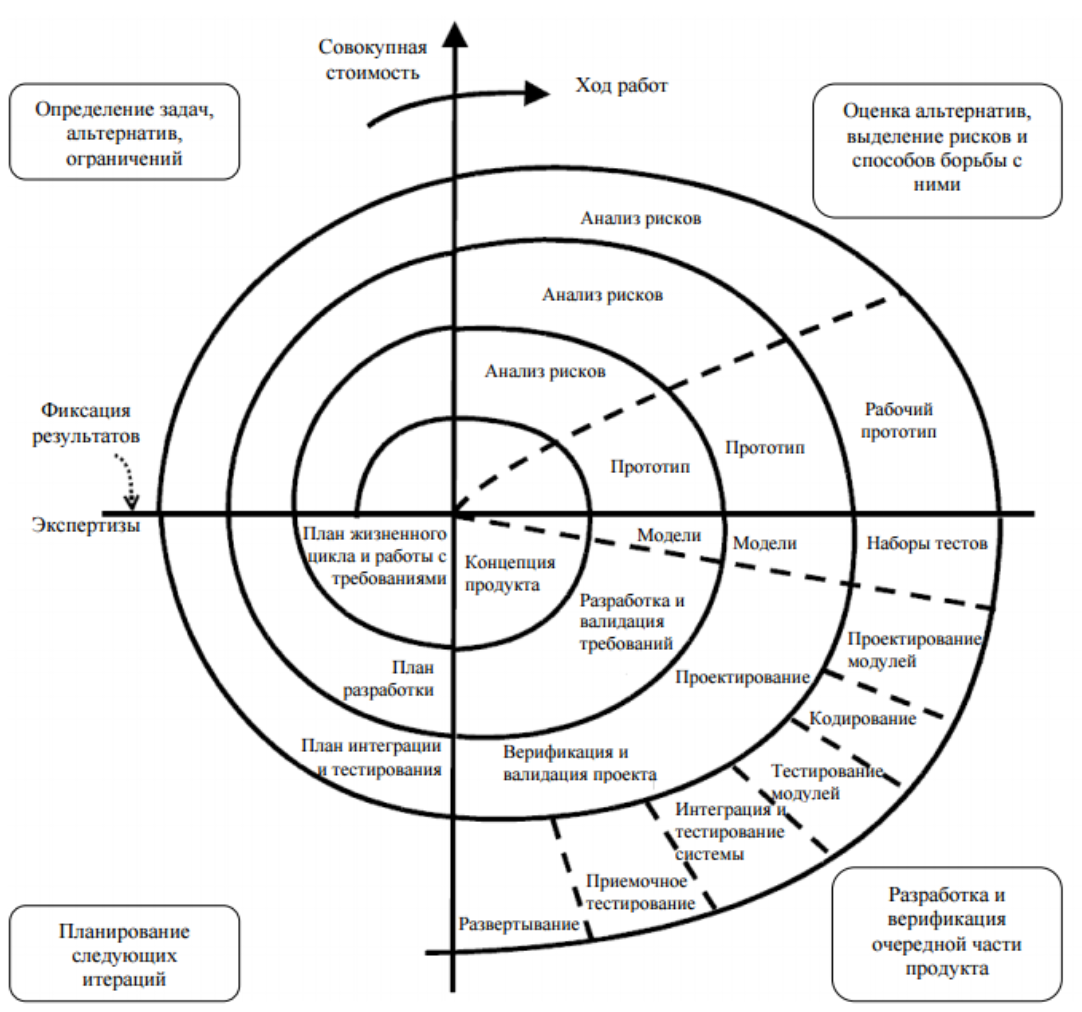
\includegraphics[width=0.7\textwidth]{spiralModel.png}
\end{center}

Название <<спиральной>> эта модель получила из-за изображения хода работ в <<полярных координатах>>, в которых угол соответствует выполняемому этапу в рамках общей структуры итераций, а удаление от начала координат~--- затраченным ресурсам. Каждый виток спирали соответствует созданию фрагмента или версии ПО. Дополнительное преимущество: на каждом витке спирали можно собрать метрические характеристики проекта (трудоемкость затрат, затраты на проект, длительность, документированность). Таким образом уточняется план-график дальнейшей работы.

Заметим, что спиральная модель может применяться на довольно высоком уровне абстракции: например, за квадрантом конструирования может скрываться целый жизненный цикл производства ПО новой версии.

Для применения этой модели может быть несколько причин:

\begin{itemize}
    \item необходимость предупреждения рисков и быстрого реагирования на них;
    \item необходимость предоставлять заказчику частичные версии проектов для получения отзывов и пожеланий.
\end{itemize}

Минусы:

\begin{itemize}
    \item требуется более искусное управление;
    \item трудности в определении момента перехода на следующий этап;
    \item необходимость поддержки целостности архитектуры;
    \item слишком большое количество витков потребует увеличения затрат на вспомогательную работу (планирование, рефакторинг и  т.п.).
\end{itemize}

В отличие от водопадной модели, в спиральной нет предопределенного и обязательного набора витков. Каждый виток может стать последним при разработке системы, при его завершении составляются планы следующего витка. Наконец, виток является именно фазой, а не видом деятельности, как в водопадной модели, в его рамках может осуществляться много различных видов деятельности, то есть модель является двумерной.

Ещё одним примером спиральной модели является модель Эрика Рисса\footnote{\url{https://www.ozon.ru/context/detail/id/18322266/} (дата обращения: 25.02.2023).}. Модель итерационная, состоящая из трех этапов. Каждый этап дает на выходе артефакт, используемый в следующем этапе. 

\begin{center}
    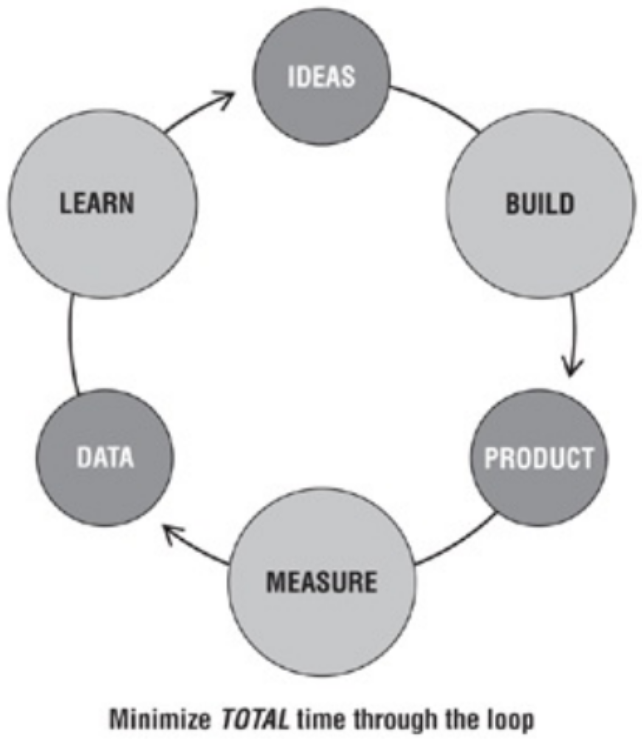
\includegraphics[width=0.3\textwidth]{theLeanStartupModel.png}
\end{center}

На этапе создания создается или изменяется разрабатываемый продукт. При этом основная задача данного этапа~--- создание <<минимального ценного (для покупателя) продукта>> (MVP). Как только такой продукт, удовлетворяющий основным требованиям к функциональности, создаётся, он передаётся на следующую фазу. На фазе измерений продукт оценивается покупателями (например, с помощью A/B тестирования) и экспертами. На фазе изучения данные тестирований расшифровываются и на основе их создаются новые требования к следующей версии продукта.

Модель довольно простая и в этом главное её достоинство. Она нацелена на постоянную адаптацию хода проекта под изменяющиеся условия и может применяться не только при разработке ПО, но и вообще при разработке любого нового продукта, разработка которого связана с высокой степенью риска.

Далее рассмотрим несколько более конкретных методологий разработки. 

\section{Rational Unified Process (RUP)}

Унифицированный процесс Rational (Rational Unified Process, RUP) является примером так называемого <<тяжелого>> процесса, детально описанного и предполагающего поддержку собственно разработки исходного кода ПО большим количеством вспомогательных действий. Примерами подобных действий являются разработка планов, технических заданий, многочисленных проектных моделей, проектной документации, и пр.

Основная цель такого процесса~--- отделить успешные практики разработки и сопровождения ПО от конкретных людей, умеющих их применять. Многочисленные вспомогательные действия дают надежду сделать возможным успешное решение задач по конструированию и поддержке сложных систем с помощью имеющихся работников, не обязательно являющихся суперпрофессионалами.

Для достижения этого выполняется иерархическое пошаговое детальное описание предпринимаемых в той или иной ситуации действий, чтобы можно было научить обычного работника действовать аналогичным образом. В ходе проекта создается много промежуточных документов, позволяющих разработчикам последовательно разбивать стоящие перед ними задачи на более простые. Эти же документы служат для проверки правильности решений, принимаемых на каждом шаге, а также отслеживания общего хода работ и уточнения оценок ресурсов, необходимых для получения желаемых результатов.

Исторически RUP является развитием модели процесса разработки, принятой в компании Ericsson в 70-х–80-х годах XX века. Эта модель была создана Иваром Якобсоном (Ivar Jacobson), впоследствии, в 1987, основавшим собственную компанию Objectory AB именно для развития технологического процесса разработки ПО как отдельного продукта, который можно было бы переносить в другие организации. После вливания Objectory в Rational в 1995 разработки Якобсона были интегрированы с работами Ройса, Крухтена (Philippe Kruchten) и Буча (Grady Booch), а также с развивавшимся параллельно универсальным языком моделирования (Unified Modeling Language, UML).

RUP основан на трех ключевых идеях.

\begin{itemize}
    \item Весь ход работ направляется итоговыми целями проекта, выраженными в виде вариантов использования (use cases)~--- сценариев взаимодействия результирующей программной системы с пользователями или другими системами, при выполнении которых пользователи получают значимые для них результаты и услуги. Разработка начинается с выделения вариантов использования и на каждом шаге контролируется степенью приближения к их реализации.
    \item Основным решением, принимаемым в ходе проекта, является архитектура результирующей программной системы. Архитектура устанавливает набор компонентов, из которых будет построено ПО, ответственность каждого из компонентов (т.е. решаемые им подзадачи в рамках общих задач системы), четко определяет интерфейсы, через которые они могут взаимодействовать, а также способы взаимодействия компонентов друг с другом. Архитектура является одновременно основой для получения качественного ПО и базой для планирования работ и оценок проекта в терминах времени и ресурсов, необходимых для достижения определенных результатов. Она оформляется в виде набора графических моделей на языке UML.
    \item Основой процесса разработки являются планируемые и управляемые итерации, объем которых (реализуемая в рамках итерации функциональность и набор компонентов) определяется на основе архитектуры.
\end{itemize}

RUP выделяет в жизненном цикле 4 основные фазы, в рамках каждой из которых возможно проведение нескольких итераций. Кроме того, разработка системы может пройти через несколько циклов, включающих все 4 фазы.

\begin{enumerate}
    \item Фаза начала проекта. Основная цель этой фазы~--- достичь компромисса между всеми заинтересованными лицами относительно задач проекта и выделяемых на него ресурсов. На этой стадии формируется техническое задание, определяются основные цели проекта, руководитель и бюджет, основные средства выполнения~--- технологии, инструменты, ключевые исполнители. Также, возможно, происходит апробация выбранных технологий, чтобы убедиться в возможности достичь целей с их помощью, и составляются предварительные планы проекта.
    \item Фаза проектирования. Основная цель этой фазы~--- на базе основных, наиболее существенных требований разработать стабильную базовую архитектуру продукта, которая позволяет решать поставленные перед системой задачи и в дальнейшем используется как основа разработки системы.
    \item Фаза конструирования. Основная цель этой фазы~--- детальное прояснение требований и разработка системы, удовлетворяющей им, на основе спроектированной ранее архитектуры. В результате должна получиться система, реализующая все выделенные варианты использования.
    \item Фаза внедрения. Цель этой фазы~--- сделать систему полностью доступной конечным пользователям. На этой стадии происходит развертывание системы в ее рабочей среде, бета-тестирование, подгонка мелких деталей под нужды пользователей и т.п.
\end{enumerate}

RUP также определяет дисциплины, включающие различные наборы деятельностей, которые в разных комбинациях и с разной интенсивностью выполняются на разных фазах. В документации по процессу каждая дисциплина сопровождается довольно большой диаграммой, поясняющей действия, которые нужно выполнить в ходе работ в рамках данной дисциплины, артефакты, с которыми надо иметь дело, и роли вовлеченных в эти действия лиц. Дисциплины представлены на схеме ниже, и должны быть вам уже знакомы. 

\begin{center}
    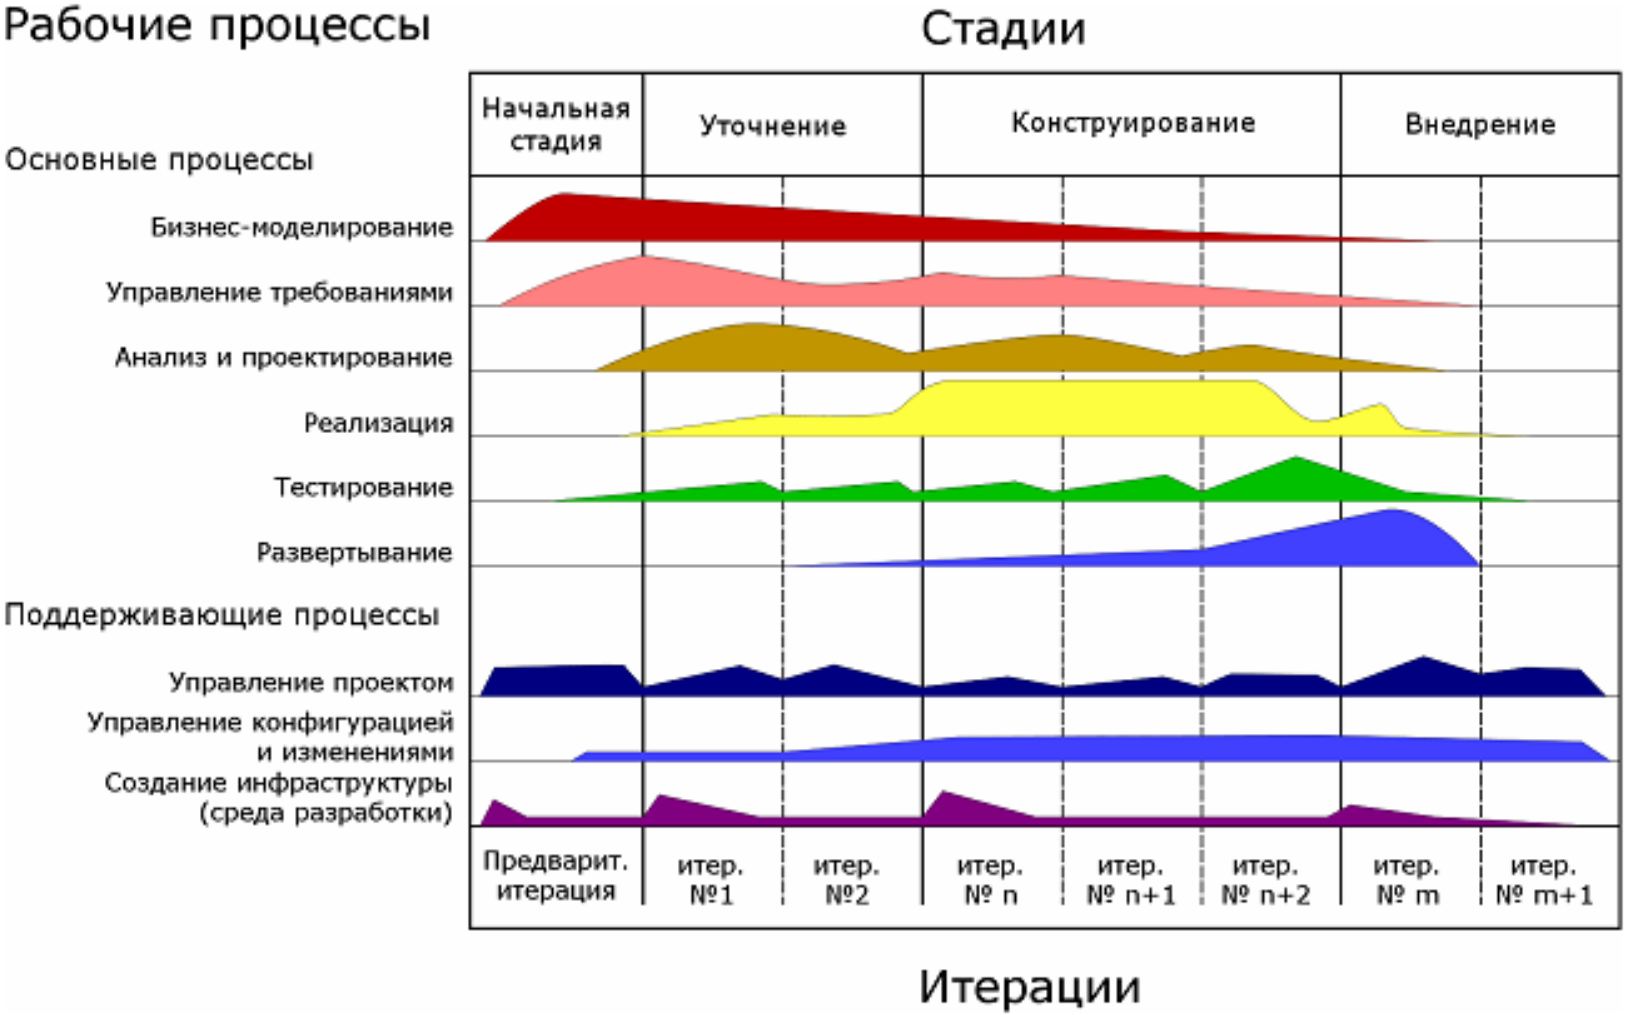
\includegraphics[width=0.7\textwidth]{rupProcesses.png}
\end{center}

Артефакты, вырабатываемые в ходе проекта, могут быть представлены в виде баз данных и таблиц с информацией различного типа, разных видов документов, исходного кода и объектных модулей, а также моделей, состоящих из отдельных элементов. Основные артефакты и потоки между ними согласно RUP изображены на рисунке ниже.

\begin{center}
    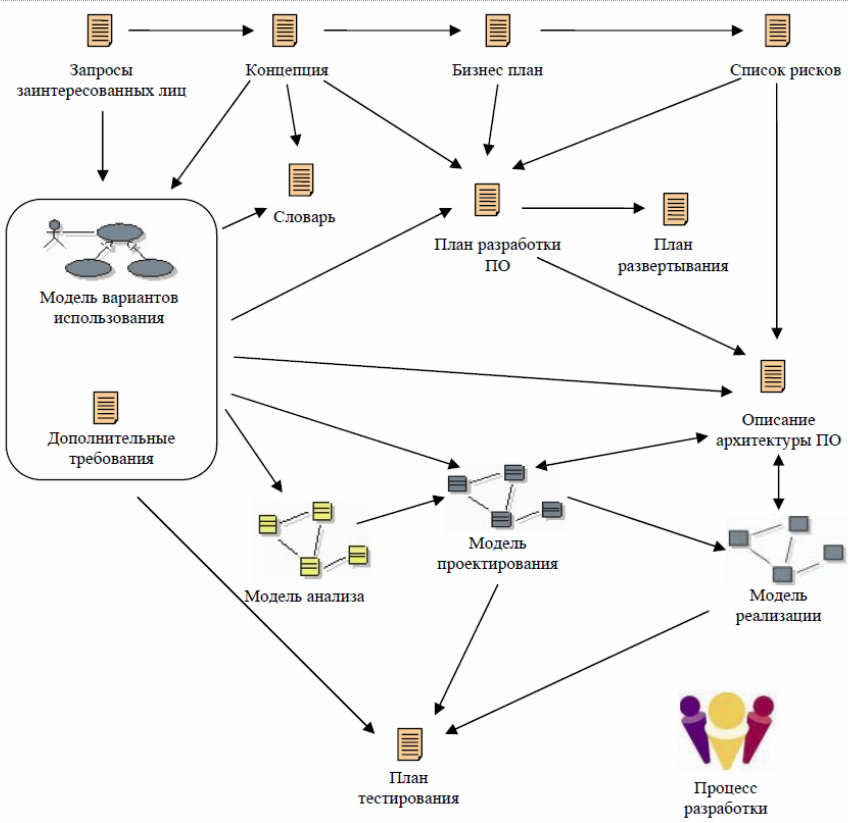
\includegraphics[width=0.9\textwidth]{rupArtefacts.png}
\end{center}

Наиболее важные с точки зрения RUP артефакты проекта~--- это модели, описывающие различные аспекты будущей системы. Большинство моделей представляют собой наборы диаграмм UML. Основные используемые виды моделей следующие.

\begin{itemize}
    \item \emph{Модель вариантов использования} определяет требования к ПО~--- то, что система должна делать~--- в виде вариантов использования. Каждый вариант использования задает сценарий взаимодействия системы с действующими лицами (actors) или ролями, дающий в итоге значимый для них результат. Действующими лицами могут быть не только люди, но и другие системы, взаимодействующие с рассматриваемой. Модель вариантов использования служит основой для проектирования и оценки готовности системы к внедрению.
    \item \emph{Модель анализа} включает основные классы, необходимые для реализации выделенных вариантов использования, а также возможные связи между классами. Эти классы представляют собой набор сущностей, в терминах которых работа системы должна представляться пользователям. Они являются понятиями, с помощью которых достаточно удобно объяснять себе и другим происходящее внутри системы, не слишком вдаваясь в детали.
    \item \emph{Модель проектирования} является детализацией и специализацией модели анализа. Она также состоит из классов, но более четко определенных, с более точным и детальным распределением обязанностей, чем классы модели анализа. Классы модели проектирования должны быть уже специализированы для конкретной используемой платформы.
    \item \emph{Модель реализации} в RUP~--- набор компонентов результирующей системы и связей между ними. Под компонентом здесь имеется в виду компонент сборки~--- минимальный по размерам кусок кода системы, который может участвовать или не участвовать в определенной ее конфигурации, единица сборки и конфигурационного управления. Связи между компонентами представляют собой зависимости между ними. Если компонент зависит от другого компонента, он не может быть поставлен отдельно от него. Часто компоненты представляют собой отдельные файлы с исходным кодом.
    \item \emph{Модель развертывания} представляет собой набор узлов системы, являющихся физически отдельными устройствами, которые способны обрабатывать информацию~--- серверами, рабочими станциями, принтерами, контроллерами датчиков и пр., со связями между ними, образованными различного рода сетевыми соединениями. Каждый узел может быть нагружен некоторым множеством компонентов, определенных в модели реализации. 
    \item \emph{Модель тестирования} задаёт сценарии работы одного или нескольких действующих лиц с системой, развивающиеся в рамках одного варианта использования.
\end{itemize}

Такая сложная организация процесса, конечно, приносит свою пользу. В теории RUP позволяет снижать риски и отслеживать возникновение новых, гибко адаптироваться к изменениям, регулярно оценивать текущее состояние и т.д. Однако, накладные расходы на поддержку этого процесса настолько велики, а сам процесс настолько сложен, что его адекватное применение возможно в очень ограниченных условиях. К тому же, мало кто захочет работать в настолько формально жестких условиях.

\subsection{Agile-подход к разработке}

Во многом как протест на всё нарастающую формализацию процесса разработки ПО стало появление методологии Agile. Это итеративная методология разработки для небольших, профессиональных, мотивированных и способных к самоорганизации команд. Наиболее полно основы Agile методологии изложены в Agile-манифесте\footnote{\url{http://agilemanifesto.org/iso/ru/manifesto.html} (дата обращения: 25.02.2023).} и в основных принципах Agile, которые и приведём ниже.

В Agile манифесте постулируется следующее:

\begin{itemize}
    \item люди и взаимодействие важнее процессов и инструментов;
    \item работающий продукт важнее исчерпывающей документации;
    \item сотрудничество с заказчиком важнее согласования условий контракта;
    \item готовность к изменениям важнее следования первоначальному плану.
\end{itemize}

Фактически, авторы призывают адаптировать процесс под сложившиеся реалии, а не адаптировать реалии под процесс. Такой подход быстро снискал определенную популярность. Позже был выпущен документ, перечисляющий основные принципы Agile.

\begin{enumerate}
    \item Наивысшим приоритетом для нас является удовлетворение потребностей заказчика, благодаря регулярной и ранней поставке ценного программного обеспечения.
    \item Изменение требований приветствуется, даже на поздних стадиях разработки. Agile-процессы позволяют использовать изменения для обеспечения заказчику конкурентного преимущества.
    \item Работающий продукт следует выпускать как можно чаще, с периодичностью от пары недель до пары месяцев.
    \item На протяжении всего проекта разработчики и представители бизнеса должны ежедневно работать вместе.
    \item Над проектом должны работать мотивированные профессионалы. Чтобы работа была сделана, создайте условия, обеспечьте поддержку и полностью доверьтесь им.
    \item Непосредственное общение является наиболее практичным и эффективным способом обмена информацией как с самой командой, так и внутри команды.
    \item Работающий продукт~--- основной показатель прогресса.
    \item Инвесторы, разработчики и пользователи должны иметь возможность поддерживать постоянный ритм бесконечно. Agile помогает наладить такой устойчивый процесс разработки.
    \item Постоянное внимание к техническому совершенству и качеству проектирования повышает гибкость проекта.
    \item Простота~--- искусство минимизации лишней работы~--- крайне необходима.
    \item Самые лучшие требования, архитектурные и технические решения рождаются у самоорганизующихся команд.
    \item Команда должна систематически анализировать возможные способы улучшения эффективности и соответственно корректировать стиль своей работы.
\end{enumerate}

Последователи Agile верят, что такой подход уменьшает объем создаваемой проектной документации, повышает гибкость проекта и позволяет выпускать более технически совершенное ПО в более краткие сроки из-за того, что большая часть усилий разработчиков сосредоточена собственно на задачах разработки и удовлетворения реальных потребностей пользователей, а не на создании кучи документов и поддержания их в актуальном состоянии. Однако он предъявляет и большие требования к командам, его использующим. Для многих команд это может оказаться существенным ограничением.

Идеи Agile нашли своё воплощение в целом ряде методик и методологий разработки, из которых мы рассмотрим две: Extreme Programming (XP) и Scrum.

\section{Экстремальное программирование}

По утверждению авторов XP, эта методика представляет собой не столько следование каким-то процессам или схемам действий, сколько применение комбинации набора определённых техник. В этом смысле ХР можно рассматривать как дисциплину разработки программного обеспечения. При этом каждая из этих техник доводится до своей экстремальной формы. В этом смысле можно представить себе XP как набор рукояток на пульте управления: каждая рукоятка соответствует некоторой методике, о которой из опыта известно, что она вполне эффективна, и каждая рукоятки установлена в максимально возможное положение.

Рассмотрим далее все эти практики.

\subsection{Разработка через тестирование}

<<Экстремальная>> техника тестирования, придуманная Кентом Беком. При обычном юнит-тестировании сначала пишется тестируемый код, а лишь потом тестирующий. Это довольно естественный порядок вещей, ведь в обратном порядке код даже не скомпилируется. Тем не менее, именно обратный порядок предлагается в подходе разработки через тестирование: 

\begin{enumerate}
    \item сначала пишем тест к несуществующей функциональности;
    \item проверяем, что тест не проходит (а вдруг тест написан плохо и проходит уже на этом шаге?);
    \item реализуем функциональность, написав минимум кода;
    \item убеждаемся, что тесты проходят;
    \item проводим рефакторинг созданного решения (устраняем дубликаты, выправляем архитектуру и т.п.).
\end{enumerate}

\begin{center}
    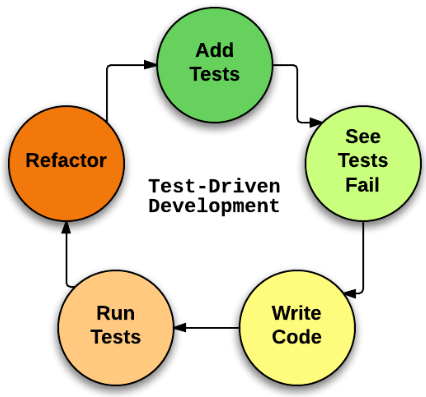
\includegraphics[width=0.45\textwidth]{tddLoop.png}
\end{center}

На самом деле данный подход не менее естественный, хоть и непривычный для большинства людей. Создавая новый модуль кода (класс, метод или что-то ещё, это не важно), вы уже знаете каким требованиям он должен соответствовать. Говоря формально, вы уже знаете предусловия и постусловия выполнения данного модуля. При этом вы еще не занялись реализацией самой функциональности и значит не будете строить предположений о модулях, которые не следуют из требований к нему. Разумно сразу записать требования к модулю в виде тестов и лишь потом начать его реализовывать.

Сюда же стоит отметить, что тесты в XP пишут все: разработчики пишут модульные и интеграционные тесты, а представители заказчика составляют функциональные тесты, проверяющие сценарии работы приложения в условиях, приближенных к реальным. Последние не обязательно должны прямо писать код, они могут готовить тестовые данные, описывать сценарии текстом и т.п.

\subsection{Заказчик всегда рядом}

Заказчик в данной методологии это не тот, кто оплачивает счета, а тот, кто может выражать интересы конечного пользователя продукта. При этом он должен быть готов взять на себя ответственность, выражая мнение пользователей. Заказчик всегда рядом~--- означает, что заказчик должен быть доступен для комментирования и обсуждения всё время работы продуктовой команды. Он участвует в процессе планирования, пишет тесты, помогает уточнять видение проекта~--- по сути является основным источником требований для разработки.

Часто даже представитель заказчика включается в команду разработки для ещё более тесного взаимодействия. Считается, что польза от такого использования его рабочего времени будет куда больше за счёт сокращения сроков разработки и повышения качества ПО.

Для многих команд это может быть одним из самых сложновыполнимых требований. В немного смягчённых условиях заказчик может не быть доступен физически, но быстро реагировать на звонки или вопросы в онлайне.

\subsection{Игра в планирование}

При игре в планирование заказчик заявляет о необходимости новой функциональности (подкрепляя это конкретными сценариями использования) и указывает её приоритетность, а разработчики оценивают её техническую выполнимость и требуемые ресурсы. Это своего рода свободные торги, в которых одна сторона называет функциональность, а другая требуемые ресурсы для её реализации. Стороны стараются прийти к выгодному решению.

Все требования описываются в виде пользовательских историй~--- небольших и понятных сценариев, позволяющих пользователям выполнить какое-то действие с системой. Каждый такой сценарий должен быть такой, чтобы его можно было оценить, чтобы было понятно, как отслеживать прогресс по его реализации, чтобы его можно было успеть реализовать за одну итерацию разработки.

Отдельно отметим важные при игре в планирование понятия идеального времени и load factor. Как правило, задача оценивается в некоторых идеальных человеко-часах. Тем не менее, в реальной жизни разработке сопутствует много другой работы, поэтому выдавать постоянно идеальное время практически невозможно. На каждой стадии развития проекта команда рассчитывает так называемый load factor (фактор загруженности) и умножает на него оценку времени выполнения задачи. Как правило, в начале проекта фактор загруженности больше (так как проводятся совещания, уточняются требования, настраивается софт и т.д.), а концу он уменьшается. Например, в начале проекта он вполне может быть равен 3, а для сработавшейся команды вполне может опускаться до 1.5-1.7.

\subsection{Парное программирование}

Это <<экстремальная>> версия ревью кода. При парном программировании над одним кодом работают сразу два программиста. Один управляет компьютером и думает над кодированием в деталях, а другой в то же время сосредоточен на общей картине. Программисты меняются ролями через заданные промежутки времени. Обычно пары формируются для решения каждой конкретной задачи из свободных и наиболее подходящих к этой задаче разработчиков.

Парное программирование позволяет писать более качественный код, так как код фактически проходит постоянную ревизию. Также такой подход позволяет увеличить продуктивность -- работая парами, программисты меньше отвлекаются на посторонние дела. Так что несмотря на кажущуюся пустую трату времени второго программиста, в итоге получается более качественный код, что позволяет сэкономить в дальнейшем на его отладке и сопровождении.

Наконец, парное программирование позволяет увеличить фактор автобуса\footnote{\url{https://en.wikipedia.org/wiki/Bus_factor} (дата обращения: 26.02.2023)} хотя бы до двух. То есть в любой момент времени в вашем коллективе есть два человека, знакомых с конкретным участком кода.

Эту практику надо использовать крайне осторожно, потому как нужно учитывать особенности не только в навыках, но и в психике и темпераменте разработчиков: идеально парное программирование работает, когда оба разработчика примерно равны и по уровню (возможно, обладая немного разной специализацией), и по темпераменту.

\subsection{Непрерывная интеграция}

Вторая группа практик нацелена на непрерывность процесса. Они широко применяются во всём мире и использование Continuous Integration буквально стало нормой для процессов современных IT-компаний и open-source проектов. Например, многие онлайн проекты выкладывает обновления своих систем по нескольку раз в день. Не всё из этого мы видим, потому что внешне может ничего и не меняться, но тем не менее.

Непрерывная интеграция означает, что интеграция новой функциональности в систему должна происходить как можно чаще: по ходу разработки нужно регулярно интегрировать свои изменения с изменениями в основной ветке разработки и убеждаться, что все тесты проходят. Если не выполнять интеграцию с достаточной частотой, вероятность возникновения конфликтов, равно как и стоимость интеграции, стремительно растет. Переход к непрерывной интеграции позволяет снизить трудоемкость интеграции и сделать её более предсказуемой за счет наиболее раннего обнаружения и устранения ошибок и противоречий.

Например, очень часто из-за несоблюдения этой практики студенческий код просто не попадает в основную кодовую базу. Выглядит это примерно так: студент берет задачу в каком-нибудь большом коллективном проекте, отводит свою ветку от основной и, как обычно, пропадает. Потом он через некоторое время объявляется и показывает свою задачу, выполненную поверх кодовой базы, которая уже успела устареть за то время, что студент делал свою задачу. И часто бывает, что такую работу приходится выкидывать просто потому, что ее интегрировать дороже, чем заново написать, а заново писать никто не хочет. Поэтому делайте интеграцию как можно чаще.

Когда Бек писал свою книгу, интеграцию приходилось выполнять вручную~--- выделялся особый компьютер, за который можно было сесть и заинтегрировать свои изменения в общий код, проверить работоспособность тестов и т.п. Современные инструментальные средства позволяют делать многое удалённо и автоматически (например, популярная в open-source сообществе система непрерывной интеграции Github Actions умеет запускать сборку проекта и запуск тестов после каждого коммита), так что внедрять эту практику в жизнь стало гораздо удобнее.

\subsection{Рефакторинг}

Подход к улучшению структурной целостности и качества кода существующих программ без изменения внешнего поведения называется рефакторингом. Каждый шаг рефакторинга прост. Это может быть перемещение поля из одного класса в другой, вынесение фрагмента кода из метода и превращение его в самостоятельный метод, или даже перемещение кода по иерархии классов. Каждый отдельный шаг может показаться элементарным, но совокупный эффект таких малых изменений в состоянии радикально улучшить проект или даже предотвратить распад плохо спроектированной программы. 

Код постоянно меняется, часто в экстренных условиях, и рефакторинг~--- это такая практика, которая позволяет поддерживать код в хорошем состоянии. Все изменения кода направлены на то, чтобы сделать его понятнее, читабельнее, проще, сделать архитектуру лучше и т.д. Казалось бы, зачем это делать, если новой функциональности не добавляется? Но как показывает практика, вы не можете постоянно вставлять костыли в ваш код и надеяться, что он будет оставаться понятным и хорошо работающим.

Рефакторинг~--- это, по сути, процесс устранения технического долга. Чем дольше копится этот долг, тем сложнее становятся изменения, которые потом нужно будет вносить для его устранения. И зависимость тут нелинейная. Подобное верно не только для рефакторинга, схожее поведение наблюдается и в криминалистике, да и в реальной жизни~--- поддерживать порядок каждый день занимает куда меньше усилий, чем полномасштабная уборка раз в месяц. Так что рефакторинг~--- это такая вещь, которую нужно делать постоянно, а в XP он и вовсе одна из основных практик.

Идею рефакторинга можно продемонстрировать на следующей истории.

Некому Джону нужна была вывеска для магазина, в котором он производил и продавал шляпы. Придуманная им версия выглядела так:

\begin{center}
    
\includegraphics[width=0.4\textwidth]{hatsRefactoringInitial.png}
\end{center}

Перед использованием вывески Джон решил показать ее нескольким друзьям и собрать отзывы. Первый друг полагал, что слова <<шляпных дел мастер>> лишние, поскольку далее следует <<изготавливает... шляпы>>, а это значит, что Джон~--- шляпный мастер. Поэтому <<шляпных дел мастер>> было вычеркнуто. Следующий друг заметил, что слово <<изготавливает>> может быть исключено, поскольку клиентам все равно, кто изготавливает шляпы. Вычеркнули и это слово. Третий друг сказал, что, по его мнению, нет смысла писать <<за наличный расчет>>, т.к. шляпы обычно не продают в кредит. Предполагается, что шляпы покупают за деньги. Эти слова также были опущены.

Теперь вывеска гласила: <<Джон Томпсон продает шляпы>>.

<<Продает шляпы!>>~--- сказал еще один друг,~--- <<Да ведь никто и не ожидает, что ты будешь раздавать их даром. Какая тогда польза от этого слова?>> <<Продает>> было вычеркнуто. К этому моменту не было никакой пользы от слова <<шляпы>>, т.к. шляпа была нарисована на вывеске. Итак, в конечном счете, вывеска сократилась до такой:

\begin{center}
    
\includegraphics[width=0.2\textwidth]{hatsRefactoringFinal.png}
\end{center}

Эта вывеска проще, компактнее и дешевле в производстве. Вот и с кодом при рефакторинге происходят похожие вещи.

\subsection{Частые небольшие релизы}

Суть практики в том, что версии/релизы продукта должны поступать в эксплуатацию как можно чаще. Чем раньше заказчик приступит к эксплуатации продукта, тем раньше разработчики получат от него информацию о том, соответствует ли новая версия продукта требованиям заказчика. Эта информация может оказаться чрезвычайно полезной при планировании следующего выпуска. Ну и чем раньше версия дойдёт до пользователей, тем раньше мы начнём зарабатывать на этом ПО.

Важность этой практики настолько велика, что в конце каждой итерации делается новый релиз независимо от того, сделан ли весь запланированный объём работы или нет. То, что доделать или проверить не успели, попадает в следующий релиз, если будет еще актуально, а версия будет выдана заказчику в любом случае.

\subsection{Простота архитектуры}

Данная практика гласит, что в каждый момент архитектура системы должна быть максимально простой. То есть,

\begin{enumerate}
    \item выполняются все тесты,
    \item нет дублирующейся логики (включая скрытое дублирование, например, посредством параллельных иерархий классов),
    \item выражается каждая из идей, важных для программистов,
    \item существует наименьшее возможное количество классов и методов.
\end{enumerate}

Каждый фрагмент дизайна системы должен доказать свое право на существование на основании всех перечисленных правил. Эта практика может противоречить тому, что обычно рассказывают в курсах по архитектуре, когда проектирование понимают как деятельность, направленную на будущее. Однако XP говорит нам, что если будущее в неопределенности, значит, включение в архитектуру функциональности только на основании абстрактных размышлений выглядит безумством. Добавляйте в дизайн то, что вам нужно, и только тогда, когда это действительно вам нужно, говорит нам XP. И тут мы опять видим сильную зависимость применимости этих практик от уровня разработчиков в команде. Нужно обладать большим опытом, чтобы инкрементально наращивать архитектуру и сохранять её целостность. Это реально, только если в голове есть общий замысел, куда вкладываются все эти инкрементальные изменения, а начинающим разработчикам такой замысел в голове построить может быть довольно сложно.

\subsection{Метафора}

В ХР метафора во многом заменяет собой то, что другие люди называют термином <<архитектура>>. Проблема состоит в том, что архитектура~--- это, как правило, огромная по размерам схема системы, которая не дает представления о ее целостности.

Смысл метафоры в следующем: <<мы сделаем некоторое описание того, как наша система работает. Расскажем, как, кем, в каких случаях она будет использоваться. Опишем все ключевые особенности, ключевые сущности системы, пользователя. И вот это станет заменой архитектуры>>. Т.е. метафора~--- это некоторое описание. Технические специалисты и заказчики разговаривают на разных языках:  мы оперируем более техническими моментами, а заказчики хорошо понимают предметную область. Как с ними договориться? Вот здесь метафора и помогает.

\subsection{Коллективное владение кодом}

Любой член команды, который видит возможность добавить что-либо в любой раздел кода системы, может сделать это в любой подходящий для этого момент времени.

Исторически к владению кода было два подхода: полное отсутствие владения и индивидуальное владение. В давние времена различными кусками кода программы никто не владел. Если кто-либо желал изменить какой-либо код, он мог сделать это в соответствии со своими собственными пожеланиями. Результатом был хаос. Код разрастался очень быстро и с такой же скоростью он стремительно терял стабильность. Чтобы взять ситуацию под контроль, программисты стали использовать индивидуальное владение кодом. Единственным человеком, кто обладал правом внесения в некоторый фрагмент кода изменений, являлся официальный владелец этого кода. Если кто-либо, не являющийся владельцем, видел, что код необходимо изменить, он должен был обратиться с соответствующей просьбой к владельцу. В результате такой практики действительный код системы начинал расходиться с тем, каким его хотели бы видеть работающие в рамках проекта программисты. Изменение кода в рамках подобного подхода превращалось в своего рода бюрократическую процедуру: люди начинали избегать обращаться к владельцу кода для того, чтобы внести в код желаемые изменения, вместо этого они предпочитали работать с тем, что есть. В конце концов, внести изменение требуется прямо сейчас, а не спустя некоторое время. Таким образом, код оставался относительно стабильным, однако он не эволюционировал с достаточно большой скоростью. А когда владелец кода находил другую работу и уходил из команды, могли возникнуть серьезные проблемы.

В рамках ХР ответственность за весь код системы лежит на всех членах команды. Это переход к первому варианту, где все писали везде, только теперь не хаотично, а централизованно. Нельзя сказать, что каждый член команды хорошо знает каждую часть кода, однако можно сказать, что каждый член команды знает по крайней мере что-то о каждой части. Это позволяет раскидывать знания по проекту и позволяет повысить ответственность каждого разработчика за всю систему в целом. И если пара программистов работает над решением некоторой задачи и видит, что для упрощения работы требуется внести модификации в некоторую часть кода, тем самым улучшив этот код, изменения вносятся немедленно, благодаря чему решаемая этой парой задача упрощается.

Также коллективное владение препятствует проникновению сложного кода в систему. Если вы знаете, что кто-то еще кроме вас в самом ближайшем времени (буквально через несколько часов) будет просматривать код, который вы сейчас пишете, вы дважды подумаете, прежде чем добавите в систему сложный код, которому вы не можете довериться прямо сейчас. 

\subsection{Стандарты кодирования}

Если мы собираемся перебрасывать программистов с разработки одной части системы на разработку другой части системы, обеспечивать постоянный рефакторинг кода программистами, которые этот код не писали, мы просто не можем позволить себе в рамках одного проекта применение нескольких разных стилей кодирования.

В рамках XP необходимо добиться того, чтобы было сложно понять, кто является автором того или иного участка кода: вся команда работает как один человек. В каждом проекте вводятся свои стандарты, устанавливаются точные правила стиля программирования. Каждый член команды должен следовать этим правилам в процессе кодирования. В современных проектах сборка может даже считаться проваленной, если не проходит проверка стайлгайда.

\subsection{40-часовая рабочая неделя}

Последняя практика заключается в том, что работать нужно 40 часов в неделю, не больше и не меньше. Поддерживать на протяжении долгого времени некоторый темп возможно только в том случае, если этот темп комфортный. Если вы работаете 60-80 часов в неделю постоянно, то на третью неделю вы захотите что-то поменять в вашей жизни, скорее всего~--- работу.

Конечно же, необязательно, чтобы рабочих часов в неделе было ровно 40. Разные люди способны эффективно работать в течение различного времени. Один человек не может концентрировать свое внимание дольше, чем в течение 35 рабочих часов, другой способен успешно действовать в течение 45 часов в неделю. Но никто не способен работать по 70 часов в неделю на протяжении многих недель и при этом оставаться свежим, творческим, внимательным и уверенным в своих силах. А именно такие работники вам и нужны в XP-команде.

Благоприятный темп для программиста~--- это когда он приходит утром с желанием работать, а вечером уходит с небольшой усталостью, но полностью удовлетворенный результатом своей работы. И при этом в пятницу вечером он должен быть уставшим настолько, чтобы не хотеть заниматься работой до понедельника. В таком темпе хороший программист может работать бесконечно долго.

Работа во внеурочное время~--- это признак серьезных проблем планирования в проекте. В рамках ХР действует очень простое правило: нельзя работать во внеурочное время две недели подряд. В течение одной недели можно поднапрячься и поработать несколько лишних часов. Но если в очередной понедельник вы приходите на работу и объявляете <<чтобы достичь поставленных целей, мы должны снова работать допоздна>>, это означает, что у вас возникли проблемы, которые вы не сможете решить простым увеличением рабочего времени.

Переработки хороши только в коротких сроках. Если у вас через три дня дедлайн и вы понимаете, что совсем не успеваете, то вы сядете и будете писать без остановки. Но если у вас дедлайн через три месяца и вам говорят <<всё, оставшиеся три месяца живем на работе>>, надо собирать вещи и уходить. Если вы попали в команду, где переработки считаются нормой, да еще и приветствуются, уходите оттуда сразу! Какие бы вам бонусы там не обещали, вы просто себе навредите больше.

(Вот тут: \url{https://www.youtube.com/watch?v=fp-sutUbSnY} (дата обращения: 26.02.2023) доступно рассказывают про то, как формируется выгорание и какие процессы в организме вызывает. А вот тут: \url{https://www.youtube.com/watch?v=q2vVsjS3ofA} (дата обращения: 26.02.2023)~--- как это потом лечить.)

\subsection{Зависимости между практиками}

\begin{center}
    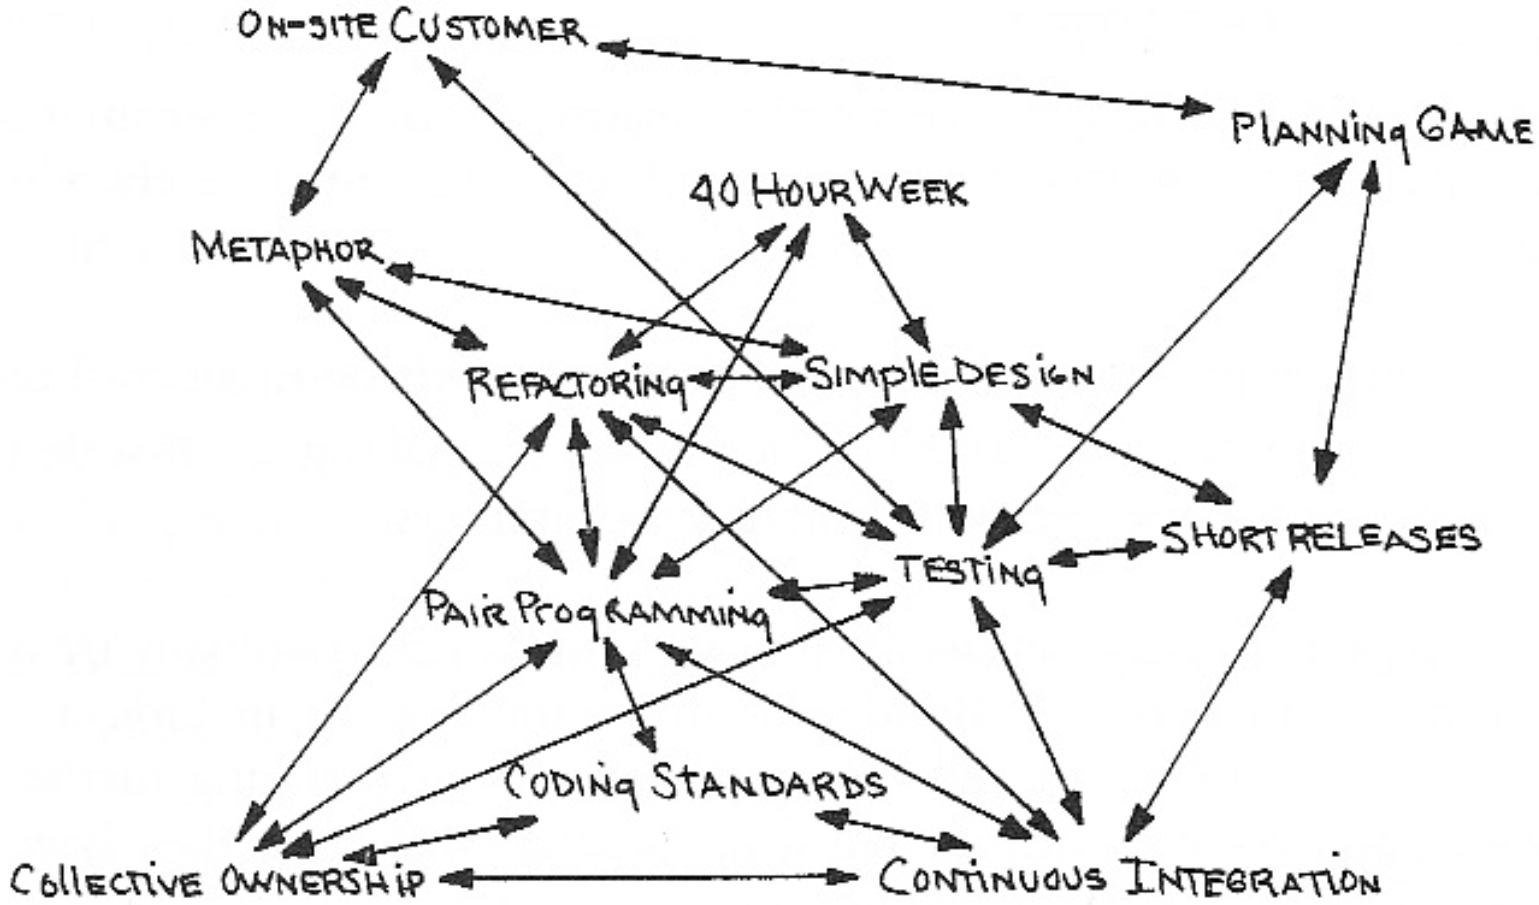
\includegraphics[width=0.7\textwidth]{xpPracticesRelationship.png}
\end{center}

На самом деле, довольно запутанная схема, но ничего тут сложного нет. Вот есть у вас короткие релизы, они очевидным образом зависят от тестирования. Если не будет тестирования, то и короткие релизы у вас тоже сломаются. Также они зависят от Continuous Integration: если у вас нет непрерывной интеграции, то и короткие релизы у вас тоже делать не получится, потому что в определенный момент может выясниться, что ваш код просто не интегрируется.

В общем, это просто зависимости между практиками. Если убрать какую-либо практику, то с большой вероятностью отвалятся те практики, которые от нее зависят. Но, например, можно убрать короткие релизы, но при этом делать тестирование. Поэтому эти двунаправленные стрелочки немного вводят в заблуждение, но, так или иначе, многие практики влияют на остальные.

\subsection{Процесс XP}

\begin{center}
    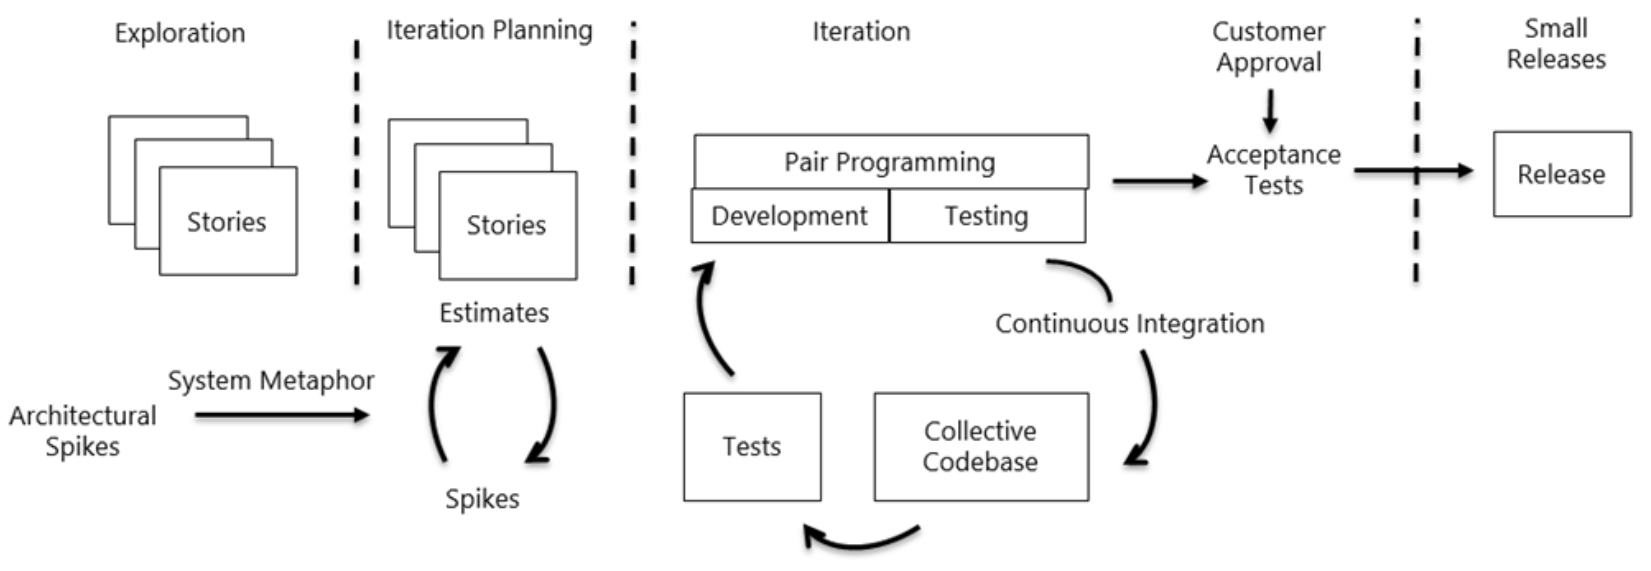
\includegraphics[width=\textwidth]{xpProcess.png}
\end{center}

С процессом все довольно очевидно: есть некая начальная фаза~--- исследование, потом вы планируете ваши итерации, затем запускаете их, тестируете, и так все идет по кругу. В конце каждой итерации запускаете приемочные тесты и делаете релиз.

\subsection{Итерации в XP}

\begin{center}
    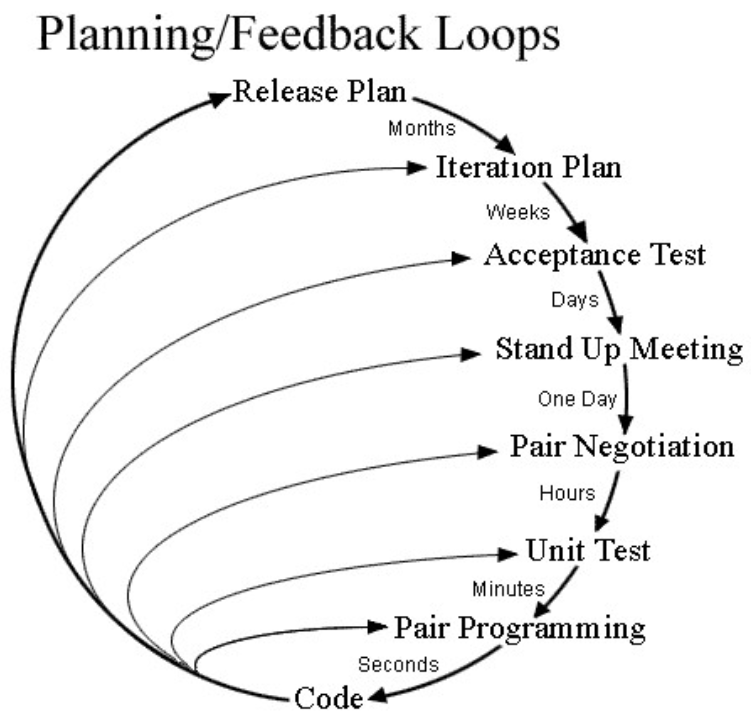
\includegraphics[width=0.5\textwidth]{xpIterations.png}
\end{center}

На этом рисунке показаны разные итерации, которые существуют в XP. Пойдем снизу: у вас есть код и у вас есть парное программирование. Вы быстро написали код, получили обратную связь от коллеги~--- итерация идет в секунды. Потом у вас есть модульные тесты, которые вы запускаете не каждую секунду, но раз в столько-то минут. Ежедневные встречи проходят раз в день. И т.д. В итоге постоянный контроль и адаптация под изменяющиеся условия.

\subsection{Применимость}

Как уже говорилось выше, XP накладывает серьезные ограничения на команду. Если вы берете пять бестолковых людей, они не смогут работать по XP. Даже два бестолковых работника в команде из пяти человек всё испортят.

ХР очень проста в своих деталях, однако ее сложно применить на практике. Методики, составляющие ХР, может изучить каждый, кто занимается программированием. Это несложная часть работы. Сложная часть~--- это собрать и поддерживать в состоянии баланса. То же парное программирование: чтобы хорошо заработало, нужно, чтобы много различных условий совпало. Но если все эти условия совпадут, вы получаете процесс, который позволяет заказчику больше вам доверять, более прозрачен ваш процесс становится для заказчика. Он тут же понимает, что происходит, он быстрее на это реагирует, у вас получается софт лучшего качества, вы не делаете лишнюю работу и т.д.

Из вышесказанного можно сделать вывод, что наилучшим образом XP находит свое применение для небольших команд, или команд, работающих с неясными или постоянно меняющимися требованиями. 

\end{document}
